\subsection*{Датчики - равномерное распределение}
\addcontentsline{toc}{subsection}{Датчики - равномерное распределение}

\textbf{Задание:}\\
Реализовать генератор случайных чисел, используя метод серединных квадратов (фон Нейман). Проанализировать свойства полученной последовательности.\\

\textbf{Решение:}\\
В методе серединных квадратов изначально задаётся количество разрядов числа $k$ и начальное значение $R_0$. Далее число $R_0$ возводится в квадрат и из середины квадрата числа берётся $k$-значное число, которое снова возводится в квадрат, и так далее.\\
Обязательным условием является то, что количество разрядов $k$ должно быть чётным числом.\\
\newline
Данный алгоритм был реализован на языке программирования Python. (Рисунок \ref{fig:mid_square_method_code})
\begin{figure}[h]
	\centering 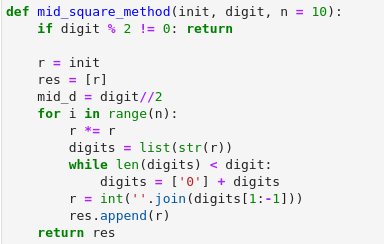
\includegraphics[scale=0.8]{mid_square_method_code}
	\caption{Реализация метода серединных квадратов}
	\label{fig:mid_square_method_code}
\end{figure}
\newpage
Алгоритм был запущен с параметрами $k = 10$, $R_0 = 31$, $n = 10$, где $n$ -- это количество сгенерированных случайных чисел. Можно проследить, что при достаточно малых разрядах и малом начальном значении быстро получается вырождение, что плохо. (Рисунок \ref{fig:mid_square_method_result})
\begin{figure}[h]
	\centering 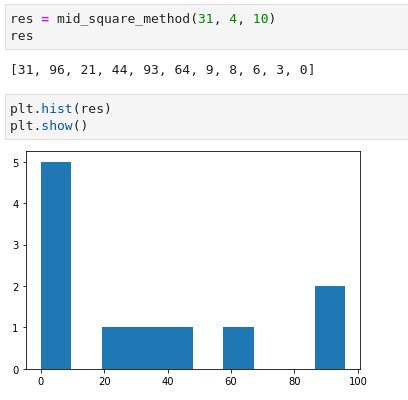
\includegraphics[scale=0.8]{mid_square_method_result}
	\caption{Результаты генерации случайных чисел методом серединных квадратов}
	\label{fig:mid_square_method_result}
\end{figure}

Также стоит проверить гипотезу о том, что получившиеся значения распределены равномерно. Для этого воспользуемся критерием Колмогорова-Смирнова. (Рисунок \ref{fig:mid_square_method_test})
\begin{figure}[h]
	\centering 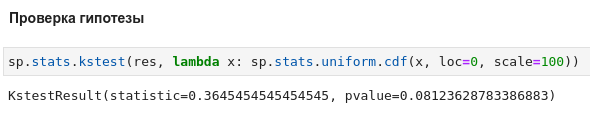
\includegraphics[scale=0.6]{mid_square_method_test}
	\caption{Результаты теста Колмогорова-Смирнова}
	\label{fig:mid_square_method_test}
\end{figure}

Значение \textit{p-value} > 0.05, значит мы принимаем гипотезу о том, что данная выборка имеет равномерное распределение.

\textbf{Задание:}\\
Реализовать линейный конгруэнтный датчик случайных чисел. Сгенерировать последовательность вещественных чисел, распределённых равномерно: 1) на интервале [0,1); \; 2) на интервале [a,b). Проанализировать полученные последовательности. Определить период, построить гистограмму.\\

\textbf{Решение:}\\
Линейный конгруэнтный метод -- это один из рекуррентных методов генерации случайных чисел. Следующий элемент последовательности может быть найден по следующей формуле:
\begin{center}
	$ r_{i+1} = (k \cdot r_i + b) \; mod \; M$
\end{center}

Линейная конгруэнтная последовательность, определённая числами $M$, $k$, $b$, $r_0$ периодична с периодом, не превышающим $M$. При этом длина периода равна $M$ тогда и только тогда, когда:
\begin{enumerate}[topsep=0pt,itemsep=-1ex,partopsep=1ex,parsep=1ex]
	\item числа $b$ и $M$ взаимно простые;
	\item $k-1$ кратно $p$ для каждого простого $p$, являющегося делителем $M$;
	\item $k-1$ кратно 4, если $M$ кратно 4.
\end{enumerate}
Сначала был реализован алгоритм для интервала [0;1) на языке программирования Python. (Рисунок \ref{fig:linear_congruent_gauge_0_1_code})
\begin{figure}[h]
	\centering 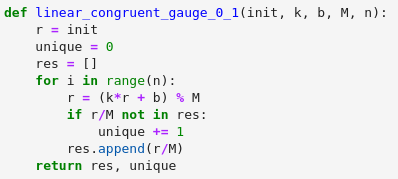
\includegraphics[scale=0.8]{linear_congruent_gauge_0_1_code}
	\caption{Реализация линейного конгруэнтного счётчика на интервале [0,1)}
	\label{fig:linear_congruent_gauge_0_1_code}
\end{figure}

\newpage
Для того чтобы получить случайные числа в интервале от [0,1) нужно поделить каждый случайный сгенерированный элемент последовательности на $M$. Также данная функция выводит период сгенерированной последовательности.
\begin{figure}[h]
	\centering 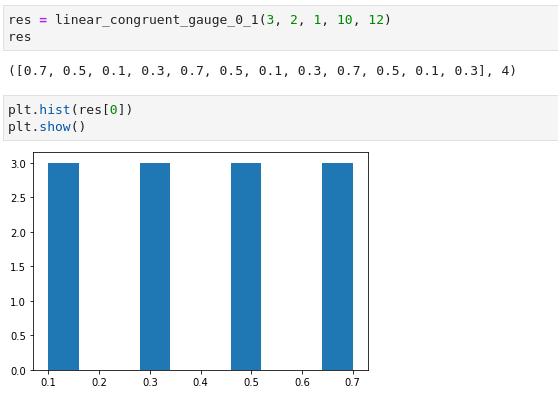
\includegraphics[scale=0.6]{linear_congruent_gauge_0_1_result}
	\caption{Результаты генерации случайных чисел линейным конгруэнтным счётчиком на интервале [0,1)}
	\label{fig:linear_congruent_gauge_0_1_result}
\end{figure}

В качестве аргументов были выбраны следующие значения: $r_0 = 3$, $k = 2$, $b = 1$, $M = 10$, $n = 12$, где $n$ -- это количество сгенерированных случайных чисел. Можно видеть, что при данном наборе аргументов длина периода составила 4. (Рисунок \ref{fig:linear_congruent_gauge_0_1_result})\\

Также стоит проверить гипотезу о том, что получившиеся значения распределены равномерно. Для этого воспользуемся критерием Колмогорова-Смирнова. (Рисунок \ref{fig:linear_congruent_gauge_0_1_test})
\begin{figure}[h]
	\centering 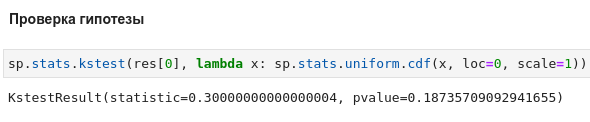
\includegraphics[scale=0.6]{linear_congruent_gauge_0_1_test}
	\caption{Результаты теста Колмогорова-Смирнова}
	\label{fig:linear_congruent_gauge_0_1_test}
\end{figure}

Значение \textit{p-value} > 0.05, значит мы принимаем гипотезу о том, что данная выборка имеет равномерное распределение.

\newpage
Далее был реализован алгоритм для интервала [a;b). (Рисунок \ref{fig:linear_congruent_gauge_a_b_code})
\begin{figure}[h]
	\centering 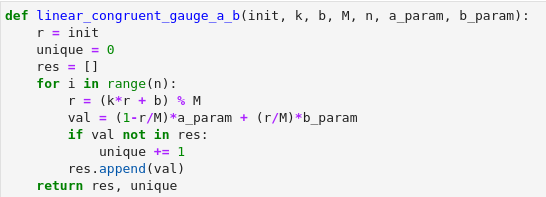
\includegraphics[scale=0.6]{linear_congruent_gauge_a_b_code}
	\caption{Реализация линейного конгруэнтного счётчика на интервале [a,b)}
	\label{fig:linear_congruent_gauge_a_b_code}
\end{figure}

Для того чтобы получить случайные числа в интервале от [a,b) нужно проделать следующее преобразование:
\begin{center}
	$(1 - \dfrac{r_i}{M})/a + \dfrac{r_i}{M} \cdot b$
\end{center}
То есть сначала мы генерируем числа в интервале от [0,1), а дальше преобразуем их к интервалу от [a,b).
\begin{figure}[h]
	\centering 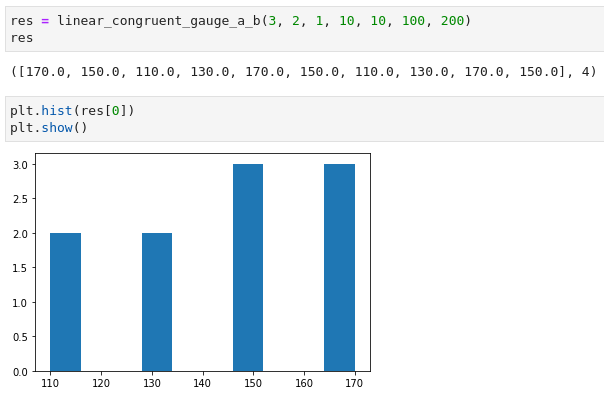
\includegraphics[scale=0.52]{linear_congruent_gauge_a_b_result}
	\caption{Результаты генерации случайных чисел линейным конгруэнтным счётчиком на интервале [a,b)}
	\label{fig:linear_congruent_gauge_a_b_result}
\end{figure}
\newpage
В качестве аргументов были выбраны следующие значения: $r_0 = 3$, $k = 2$, $b = 1$, $M = 10$, $n = 10$, $a_{param} = 100$, $b_{param} = 200$, где $n$ -- это количество сгенерированных случайных чисел. Можно видеть, что при данном наборе аргументов длина периода составила 4. (Рисунок \ref{fig:linear_congruent_gauge_a_b_result})\\

Также стоит проверить гипотезу о том, что получившиеся значения распределены равномерно. Для этого воспользуемся критерием Колмогорова-Смирнова. (Рисунок \ref{fig:linear_congruent_gauge_a_b_test})
\begin{figure}[h]
	\centering 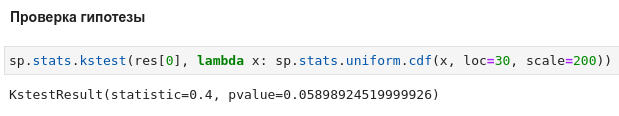
\includegraphics[scale=0.6]{linear_congruent_gauge_a_b_test}
	\caption{Результаты теста Колмогорова-Смирнова}
	\label{fig:linear_congruent_gauge_a_b_test}
\end{figure}

Значение \textit{p-value} > 0.05, значит мы принимаем гипотезу о том, что данная выборка имеет равномерное распределение.